\begin{figure*}[t]
    \centering
    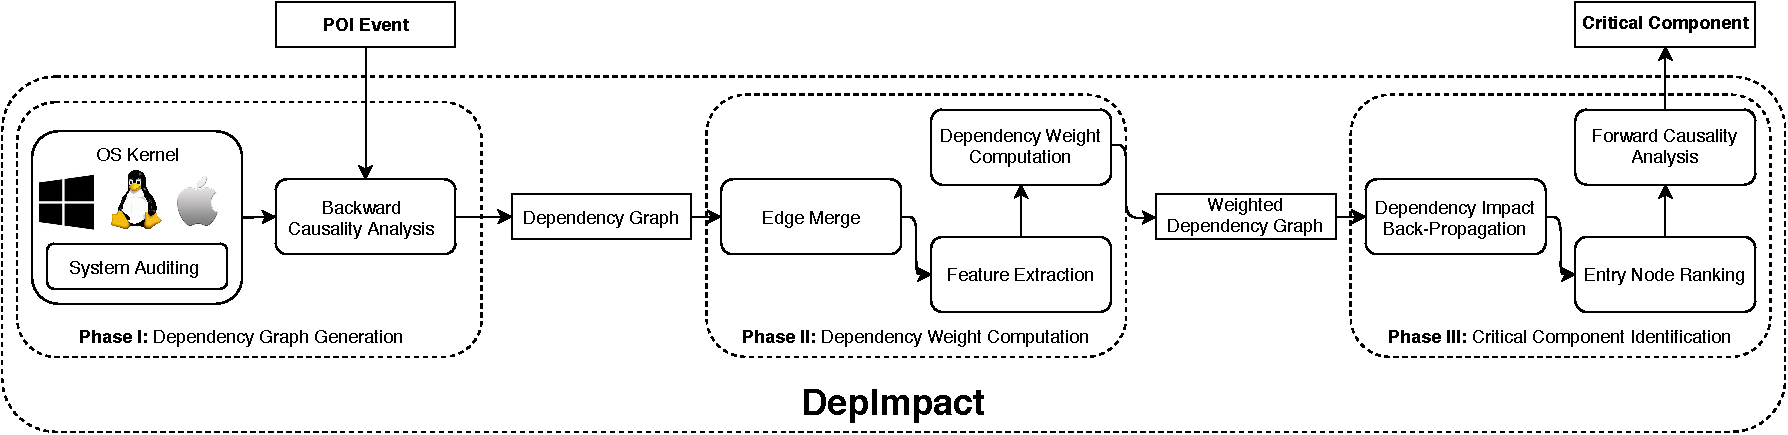
\includegraphics[width=0.95\textwidth,clip]{figs/architecture.pdf}
    \caption{Architecture of \tool}
    \label{fig:architecture}
\end{figure*}


\section{Overview}
\label{sec:overview}

%https://drive.google.com/file/d/1RE_n6d_rl2ciDsmN1IP0uVZJYl30NIG0/view?usp=sharing


\cref{fig:architecture} shows the architecture of \tool.
%
Given a POI event, \tool employs automated techniques to identify the critical component of the dependency graph for the POI event produced by causality analysis.
%
\tool consists of three phases: (1) dependency graph generation, (2) dependency weight computation, and (3) critical component identification.
%
In Phase I, \tool leverages mature system auditing frameworks~\cite{auditd,etw,dtrace,sysdig}
%(\eg auditd~\cite{auditd}, ETW~\cite{etw}, DTrace~\cite{dtrace}, and Sysdig~\cite{sysdig}) 
to collect system-level audit logs about system calls (\cref{subsubsec:system-auditing}).
Given a POI event, \tool parses the collected logs and performs backward causality analysis~\cite{backtracking,backtracking2} to generate a backward dependency graph for the POI event. (\cref{subsubsec:backward-causality}).

%
In Phase II, \tool first employs state-of-the-art dependency graph reduction techniques~\cite{reduction} to reduce the graph size
%by merging the same type of edges between two nodes that occur within a time window threshold 
(\cref{subsubsec:edge-merge}).
Then, \tool extracts features for edges (\cref{subsubsec:feature-extraction})
%that model the relevance of the edge to POI , 
and employs a discriminative feature projection scheme based on LDA to compute dependency weights (\cref{subsubsec:weight-computation}) from the features, so that critical edges can be better revealed.
The output of Phase II is a weighted dependency graph for the POI event.

%
In Phase III, \tool first employs a weighted score propagation scheme to
propagate the dependency impact from the POI event 
%(score $1.0$) 
backward along the edges to all entry nodes (\cref{subsubsec:propagation}).
Then, \tool ranks entry nodes based on their dependency impacts and selects the top candidates (\cref{subsubsec:entry-ranking}).
Finally, \tool performs forward causality analysis from the top-ranked entry nodes and identifies the overlap of the backward dependency graph and the forward dependency graph as the critical component for output (\cref{subsubsec:forward-causality}). 
Compared with the original backward dependency graph, the critical component well preserves the information that is critical to attack investigation (critical edges and attack entries) at a reduced size.




\myparatight{Threat Model}
Our threat model is similar to the threat model of previous work on system monitoring~\cite{backtracking,backtracking2,loggc,gao2018aiql,gao2018saql,liu2018priotracker,hassan2019nodoze}. 
We assume that kernel and kernel-layer auditing framework~\cite{auditd,etw,dtrace,sysdig} are part of our trusted computing base (TCB), and existing software and kernel hardening techniques~\cite{trustkernel,tamperlog} can be used to secure log storage.
Any kernel-level attack that deliberately compromises security auditing systems is beyond the scope of this work.
We assume an outside attacker that attacks the system remotely (from outside of the system). Thus, the attacker either utilizes the vulnerabilities in the system or convinces the user to download a file with malicious payload.

We do not consider the attacks performed using implicit flows (\eg side channels) that do not go through kernel-layer auditing and thus cannot be captured by the underlying provenance tracker, 
We also do not consider Mimicry attacks~\cite{mimicry} where attackers deliberately evade intrusion detection systems through a chain of events that seem benign in enterprises. 
Existing intrusion detection systems~\cite{securitybook,intrusionbook,netwrix} often relies on heuristics or analysis based on the properties of a single event, and thus are vulnerable for such attack.
While detecting Mimicry attacks is the limitation of the detection systems, it is beyond the scope of this work since our focus is to identify the relevant events as the contextual information for the alerts generated by the detection systems.



\eat{
The attacker executes APT attacks involving multiple steps such as target discovery and data exfiltration. We assume an outside attacker that attacks the system remotely (from outside of the system). Thus, the attacker either utilizes the vulnerabilities in the system or convinces the user to download a file. The main goal of the attacker is to inject her malicious files into the victim’s system without being detected. In this work, we assume the attacker does not know how the proposed reputation system operates, and hence we do not consider the potential attacks against the reputation system. 

% We do consider that insiders or external attackers have full knowledge of the deployed \tool queries and the anomaly models. 
}
